\documentclass[10pt,landscape]{scrartcl}
\usepackage{multicol}
\usepackage{calc}
\usepackage{ifthen}
\usepackage[landscape]{geometry}
\usepackage{amsmath,amsthm,amsfonts,amssymb}
\usepackage{color,graphicx}
\usepackage{hyperref}
\usepackage[font=scriptsize,labelfont=bf]{caption}
\usepackage{wrapfig}
\usepackage{graphicx,calc}
\usepackage{empheq}
\usepackage{xcolor}
%\usepackage{pbox}

\pdfinfo{
  /Title (Analysis III - PDE)
  /Creator (TeX)
  /Producer (pdfTeX 1.40.0)
  /Author (Noah Huetter)
  /Subject (Analysis III - PDE)
  /Keywords (Analysis, ETH, PDE)}


\definecolor{section}{RGB}{28,82,83}
\definecolor{titletext}{RGB}{0,0,0}
\definecolor{formula}{RGB}{249,220,155}

\setkomafont{section}{\mysection}
\newcommand{\mysection}[1]{%
    \Large\bf%
    \setlength{\fboxsep}{0cm}%already boxed
    \fcolorbox{black}{gray!40}{%
        \begin{minipage}{\linewidth}%
            \vspace*{2pt}%Space before
            #1
            \vspace*{2pt}%Space after
        \end{minipage}%
    }}

% This sets page margins to .5 inch if using letter paper, and to 1cm
% if using A4 paper. (This probably isn't strictly necessary.)
% If using another size paper, use default 1cm margins.
\ifthenelse{\lengthtest { \paperwidth = 11in}}
    { \geometry{top=.5in,left=.5in,right=.5in,bottom=.5in} }
    {\ifthenelse{ \lengthtest{ \paperwidth = 297mm}}
        {\geometry{top=1cm,left=1cm,right=1cm,bottom=1cm} }
        {\geometry{top=1cm,left=1cm,right=1cm,bottom=1cm} }
    }

% Turn on simple page number
\pagestyle{plain}

% Redefine section commands to use less space
\makeatletter
% \renewcommand{\section}{\@startsection{section}{1}{0mm}%
%                                 {-1ex plus -.5ex minus -.2ex}%
%                                 {0.5ex plus .2ex}%x
%                                 {\normalfont\large\bfseries}}
\renewcommand{\subsection}{\@startsection{subsection}{2}{0mm}%
                                {-1explus -.5ex minus -.2ex}%
                                {0.5ex plus .2ex}%
                                {\normalfont\normalsize\bfseries}}
\renewcommand{\subsubsection}{\@startsection{subsubsection}{3}{0mm}%
                                {-1ex plus -.5ex minus -.2ex}%
                                {1ex plus .2ex}%
                                {\normalfont\small\bfseries}}
\makeatother

% bring the old commands back as needed via:
\makeatletter
\DeclareOldFontCommand{\rm}{\normalfont\rmfamily}{\mathrm}
\DeclareOldFontCommand{\sf}{\normalfont\sffamily}{\mathsf}
\DeclareOldFontCommand{\tt}{\normalfont\ttfamily}{\mathtt}
\DeclareOldFontCommand{\bf}{\normalfont\bfseries}{\mathbf}
\DeclareOldFontCommand{\it}{\normalfont\itshape}{\mathit}
\DeclareOldFontCommand{\sl}{\normalfont\slshape}{\@nomath\sl}
\DeclareOldFontCommand{\sc}{\normalfont\scshape}{\@nomath\sc}
\makeatother


% make smaller enumerates
\usepackage{enumitem}
\setlist[enumerate]{itemsep=-1mm,leftmargin=3mm}

% Define BibTeX command
\def\BibTeX{{\rm B\kern-.05em{\sc i\kern-.025em b}\kern-.08em
    T\kern-.1667em\lower.7ex\hbox{E}\kern-.125emX}}

% Don't print section numbers
\setcounter{secnumdepth}{2}


\setlength{\parindent}{0pt}
\setlength{\parskip}{1pt plus 0.5ex}


%My Environments
\newtheorem{example}[section]{Example}
% -----------------------------------------------------------------------
\newcommand{\eqn}[3]
{
  \begin{minipage}[#1]{#2}
    \[ #3 \]
  \end{minipage}
}
\newcommand{\feqn}[3]
{
\fbox{
  \begin{minipage}[#1]{#2}
    \[ #3 \]
  \end{minipage}
}
}
% equation box        
\newcommand{\eqbox}[1]{\fcolorbox{black}{formula}{\hspace{0.5em}$\displaystyle#1$\hspace{0.5em}}}

\newcommand{\Pabl}[2] {\frac{\partial#1}{\partial#2}}
\newcommand{\MATR}[1]{ \displaystyle \left( \begin{matrix} #1 \end{matrix} \right)}
\newcommand{\MATRABS}[1]{ \displaystyle \left| \begin{matrix} #1 \end{matrix} \right|}
\newcommand{\Int}{\int\limits}
\newcommand\warning{%
 \makebox[1.4em][c]{%
 \makebox[0pt][c]{\raisebox{.1em}{\small!}}%
 \makebox[0pt][c]{\color{red}\Large$\bigtriangleup$}}}%

\begin{document}
\raggedright
\footnotesize
\begin{multicols*}{2}



% multicol parameters
% These lengths are set only within the two main columns
%\setlength{\columnseprule}{0.25pt}
\setlength{\premulticols}{1pt}
\setlength{\postmulticols}{1pt}
\setlength{\multicolsep}{1pt}
\setlength{\columnsep}{2pt}

\begin{center}
     \Large{\underline{Analysis III - PDE}} \\
\end{center}
% -----------------------------------------------------------------------
\IfFileExists{../build/revision.tex}{
  \input{../build/revision.tex}
  Author: Noah Huetter \hfill Date: \compiledate \hspace{1em} Commit: \revision
}{Author: Noah Huetter}

% -----------------------------------------------------------------------

% -----------------------------------------------------------------------
\vspace{2mm} \hrule
\section{General}

\subsection{Derivative Rules}
\begin{tabular}{l l l}
  Product Rule & $\frac{d}{dx}f(x)g(x)$  & = $f(x)g'(x) + f'(x)g(x)$ \\
  Chain Rule & $\frac{d}{dx}f(g(x))$     & = $f’(g(x))g’(x) $
\end{tabular}


\subsection{Some ODE}
\begin{align*}
  % &\textbf{First order} \\
  &x' + ax = c & x &= c_1 e^{-ax} + \frac{c}{a} \\
  % &\textbf{Second order} \\
  &ax'' + bx' + cx = 0 & b^2 &> 4ac &  x &= a_1 e^{\lambda_1 x} + a_2 e^{\lambda_2 x} &
  &\lambda_{1,2} = \frac{-b\pm\sqrt{b^2-4ac}}{2a} \\
  &ax'' + bx' + cx = 0 & b^2 &= 4ac &  x &= (a_1 + a_2x) e^{\lambda x} &
  &\rho =\frac{b}{2a} \\
  &ax'' + bx' + cx = 0 & b^2 &< 4ac &  x &= a_1e^{\rho t}\cos(\omega t)+a_2e^{\rho t}\sin(\omega t) &
  &\omega = \left| \frac{\sqrt{b^2-4ac}}{2a} \right|\\
\end{align*}

\subsection{Some PDE}
Using $\frac{\partial }{\partial t}x(t,s) = x'(t)$ partial derivatives. Further $x = x(t,s)$, $y = y(t,s)$

\begin{tabular}{l l l}
  \textbf{First order} & & \\
  % $ax + x' = 0$ & & $x = c_1e^{ax}$\\
  $x' = x^2 $&$ x = \frac{1}{c_1 - t} $ \\
  $x' - tx = 0$&$x = c(s)e^{-t^2/2}$\\
  \textbf{Rules} & & \\
  $[\log(x)]_t$ & $ = \frac{x_t}{x}$ \\
  % $$&$$\\
\end{tabular}

\subsection{Solve linear ODE with Integrating Factor}
Problem: \eqbox{y' + p(t)y = q(t)}
the ODE can be solved using an integrating factor $\mu(t)$

\begin{tabular}{l l}
  1. Calculate integrating factor &
    $\mu(t)=e^{\int p(t)dt}$ \\
  2. Multiply both sides of the ODE by $\mu(t)$ &
    $\mu(t)\left[y'+p(t)y\right]=\mu(t)q(t)$ \\
  3. Calculate &
    $(\mu(t)y)' = \mu(t)q(t)$ \\
  4. Integrating each side with respect to $t$ &
    $\mu(t)y = \int \mu(t)q(t)dt + C$ \\
  5. Final form &
    $y = \mu^{-1}(t) \left( \int \mu(t)q(t)dt + C \right)$
\end{tabular}


\subsection{Inequalities}
If $[a,b]$ is some interval, $f(a)<g(a)$, and $f'(x) \leq g'(x)$ on the interval, then $f(x)<g(x)$ on the interval. This implication cannot be reversed.

\subsection{Integrals}
Area of a disk $B_R$ with radius $R$ around $(x_0,y_0)$
\begin{align*}
  \int_{B_R(x_0,y_0)}u(x,y)\mathrm{d}x\mathrm{d}y &= \int_{0}^{R}\int_{0}^{2\pi}u(x_0+r\cos(\theta),y_0+r\sin(\theta)r\mathrm{d}\theta\mathrm{d}r &
\end{align*}

% -----------------------------------------------------------------------
\vfill\null
\columnbreak
\section{Notation of PDE}
unknown function $u: D \subset \mathbb{R}^n \to \mathbb{R}$

$F(x_1,x_2,\dots, x_n, u(x1_,\dots,x_n), u_{x_1}, \dots, u_{x_n}, u_{x_1 x_1}, \dots) = 0$

Short form: \eqbox{F(x)=0}

% -----------------------------------------------------------------------
\section{Classification of PDE}

\subsection{Order}
Order = order of highest derrivative in equation

\subsection{Linearity}
PDE is linear if $F$ is a linear function of the unknown function $u$

\begin{tabular}{l l l}
  \textbf{Semilinear} & \multicolumn{2}{l}{All derivatives are linear (Nonlin. only in $u$)} \\
  & \multicolumn{2}{l}{ $a(x,y,u)\frac{\partial u}{\partial x} + b(x,y,u)\frac{\partial u}{\partial y} + c(x,y)\frac{\partial^3 u}{\partial x^2 \partial y} = d(x,y,u)$ } \\
  \textbf{Quasilinear} & \multicolumn{2}{l}{Highest-order derivative are linear} \\
  & \multicolumn{2}{l}{$a(x,y,u,u+x)\frac{\partial u}{\partial x} + a(x,y,u,u_y)\frac{\partial u}{\partial y} + c(x,y,u,u_x,u_y)\frac{\partial^2 u}{\partial x^2} = d(x,y,u) $} \\
  \textbf{Linear} & linear in $u$ & $a(x,y)u_x+b(x,y)u_y=c_0(x,y)+c_1(x,y)$ \\
   & \multicolumn{2}{l}{if $u_1,u_2$ are sol. then $\lambda u_1 + (1-\lambda)u_2$ is a sol.}
\end{tabular}


\subsection{Homogeneous}
PDE is homogeneous if $F(x,y)$ = 0.

% \textbf{semi-linear}\\
% In der PDG enthaltene Ableitungen sind linear.

% \textbf{quasi-linear}\\
% In der PDG enthaltene Ableitungen h"ochster Ordnung sind linear.


% -----------------------------------------------------------------------
\section{First Order PDE: Method of Characteristics}
\subsection{Problem}
$\begin{cases}
    a(x,y,u)u_x + b(x,y,u)u_y & = c(x,y,u) \\
    u(x_0,y_0) & = f(x) \text{or} f(y)
  \end{cases}$

\subsection{Solution}
\begin{enumerate}
\item Bring to standard form 
  \begin{align*}
    a u_x + b u_y &= c
  \end{align*}

\item Parametrize initial condition 
  \begin{align*}
    x_t(t,s) &= a(x,y,u) && x(0,s) = x_0(s) \\
    y_t(t,s) &= b(x,y,u) && y(0,s) = y_0(s) \\
    u_t(t,s) &= c(x,y,u) && u(0,s) = f(s) \\
  \end{align*}

\item Solve characteristic equations
  \begin{align*}
    \frac{\partial}{\partial t}x(t,s)&=a(x,y,u) && x(0,s)=x_0(s)\\
    \frac{\partial}{\partial t}y(t,s)&=b(x,y,u) && y(0,s)=y_0(s)\\
    \frac{\partial}{\partial t}u(t,s)&=c(x,y,u) && u(0,s)=f(s)\\
  \end{align*}
  \textcolor{red}{If linked, parametrize:} $x=s\cdot\cos(t),\ y=s\cdot\sin(t)$
\item Find $s(x,y),\ t(x,y)$ and put in $u(t,s)$. Solve for $u(x,y)$ if Jacobian $J\neq0$

\end{enumerate}   

\subsection{Jacobian}
$J
= \frac{\partial (x,y)}{\partial(t,s)}
= \MATRABS{\Pabl{x}{t} & \Pabl{y}{t} \\[4pt] \Pabl{x}{s} & \Pabl{y}{s} }
= \MATRABS{a & b \\[4pt] \Pabl{x_0}{s} & \Pabl{y_0}{s} }
= (y_0)_sa - (x_0)_sb$

Must be $\neq0$ for $x,y$ to be invertable and the method of characteristics to work.

\subsection{Existence and uniqueness}
\subsubsection{Transversality condition}
For $a,b$ replace $x,y$ by $x_0,y_0$. If transversality condition is fulfilled the PDE has a unique solution. Set $t=0$.
\begin{align*}
J = \det \left(
\begin{bmatrix}
    a_0 & b_0 \\
    \frac{\partial x_0}{\partial s} & \frac{\partial y_0}{\partial s} 
  \end{bmatrix}
  \right) = (y_0)_sa - (x_0)_sb \neq 0
\end{align*}

% \textbf{Def:} Die Projektionen der charakteristischen Kurven in x,y-Ebene heissen Charakteristiken.
% \textbf{Transversalitätsbedingung (TB)} in $\Gamma(s)$:
% Projektion $\Gamma'$ von $\Gamma$ und der charakt. Kurve (Charakteristik) schneiden sich transversal 
% (Tangenten verschieden in diesem Punkt). 

% \textbf{Satz:} (erfüllt für $\det\Big(J\big(x(t,s),y(t,s)\big)\Big)|_{t=0}=\MATRABS{a & b \\[4pt] (x_0)_s & (y_0)_s }\neq0$) \\

% \begin{enumerate}
%   \item Ist die TB für $s \in [s_0, s_1] $ erfüllt, d.h. $J(s) \neq 0$, dann gibt es ein 
%   $\varepsilon > 0$ und Funktionen $x(t,s), y(t,s), u(t,s)$ definiert für $(t,s) \in (-\varepsilon,
%   \varepsilon) \times (s_0, s_1)$ welche die eindeutige Lösung des Cauchy-Problems darstellen.
%   \item Gilt $J(s) \equiv 0$ auf einem Intervall $[s_0,s_1]$, dann hat das Cauchy-Problem entweder
%   unendlich viele oder gar keine Lösungen. 
% \end{enumerate}

\subsection{Conservation law \& shock waves}

\begin{minipage}[h]{0.6\linewidth}
Considering the transport equation \eqbox{u_y+\Pabl{}{x}F(u)=0}

    $\begin{cases}
    u_y+\Pabl{}{x}F(u)=0 & {} \\
    u(x,0) = h(s) = & 
    \begin{cases}
      u^- & x \leq \alpha \\
      u^+ & x > \alpha \\
    \end{cases}
  \end{cases}$

If $u_0(s)$ is never decreasing, there will be no singularity (hence no shock wave).
\end{minipage}
\begin{minipage}[h]{0.3\linewidth}
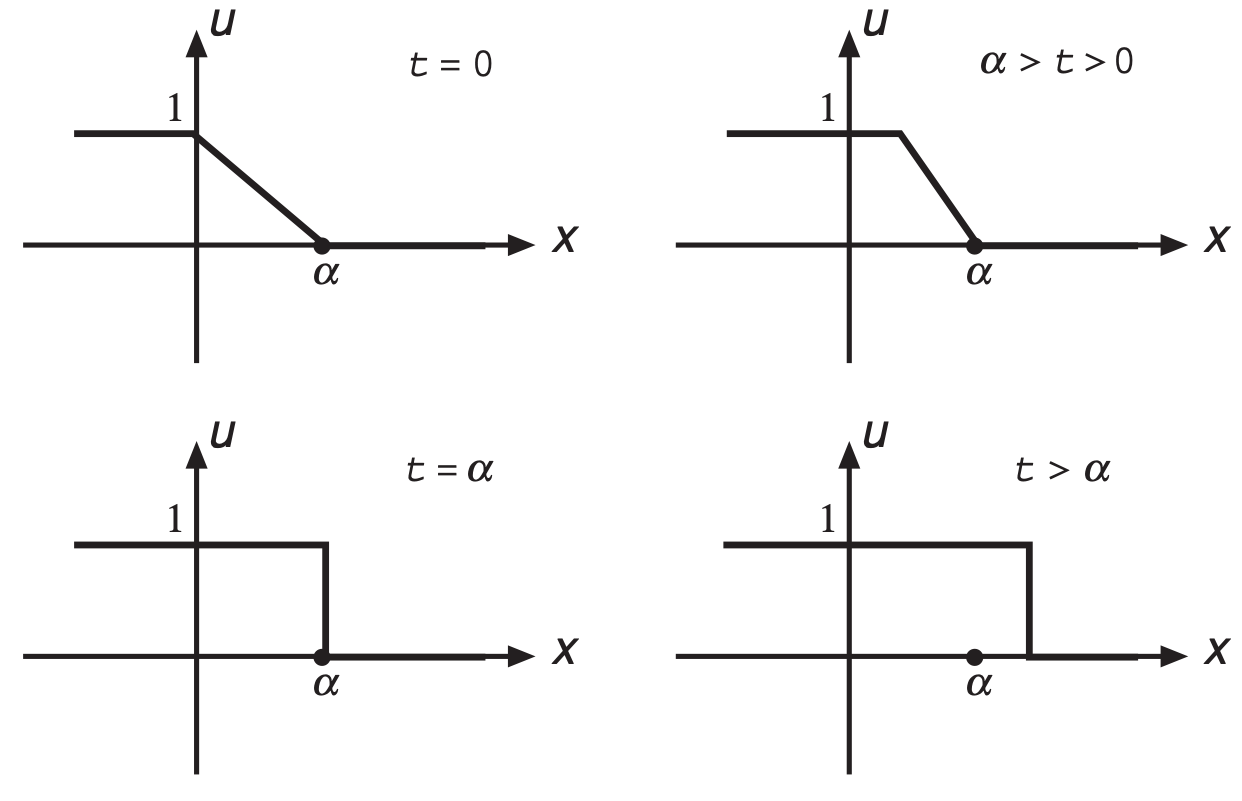
\includegraphics[width=1\linewidth]{img/shock.png}
\captionof{figure}{Several snapshots in the development of a shock wave.}
\end{minipage}

\subsubsection{Entropy Condition}
Characteristics must enter the shock curve, and are not allowed to emanate from it.
\begin{align*}
  F_u(u^-) > \gamma_y > F_u(u^+)
\end{align*}

Applying this rule to the special case $F(u)=\frac{1}{2}u^2$ we obtain that the shock solution is valid only if $u^- > u^+$.
\\
\subsubsection{Case shock wave: $u^- > u^+$} 
The characteristics intersect and it results in a shock wave. The shock wave $\gamma(y)$ describes the curve along which $u(x,y)$ assumes different values. $\gamma_y(y)$ descirbes the speed at which the discontinuity is moving (Rankine-Hugoniot condition).  The schock wave is given by
\begin{align*}
  u(x,y) &= \begin{cases} u^- & x < \gamma(y) \\ u^+ & x > \gamma(y) \end{cases} &
  \gamma_y(y) &= \frac{F(u^+) - F(u^-)}{u^+-u^-} &
  &\begin{cases} \gamma(y) = \int \gamma_y(y)dy \\ \gamma(0) = \alpha \end{cases} \\
  u^+(y) &= \lim_{x \to \gamma_y(y)_+} u(x,y) & u^-(y) &= \lim_{x \to \gamma_y(y)_-} u(x,y)
\end{align*}
$\alpha$ is the projection of the discontinuity point of the shock wave to $y = 0$.

$y_c$ denotes the critical time where the solution becomes non-smooth. That is, the classical solution is not well defined for $y>y_c$.
\begin{align*}
  y_c &= \inf_{s \in \mathbb{R}} \left\{ -\frac{1}{h'(s)} : h'(s) < 0 \right\} &
  h(s) &= u(x,0)
\end{align*}
If $h(s)$ (the initial value) has a discontinuity (e.g. a step), $y_c = 0$: the solution is weak immediately.
% \subsubsection{Case dilution wave: $u^- < u^+$} 


% -----------------------------------------------------------------------
\vfill\null
\columnbreak
\section{Second Order PDE}
\begin{align*}
  L [u] = a \cdot u_{xx} + 2b\cdot u_{xy} + c\cdot u_{yy} + d\cdot u_x + e\cdot u_y + f\cdot u = g
\end{align*}

\subsection{Classification}
Discriminant $\delta$:
\begin{align*}
  \delta(L)(x,y) &= b^2(x,y) - a(x,y)\cdot c(x,y) & L[u]
  \begin{cases}
    \text{elliptic} & \delta(L)<0 \\
    \text{parabolic} & \delta(L)=0 \\
    \text{hyperbolic} & \delta(L)>0 
  \end{cases}
\end{align*}


% -----------------------------------------------------------------------
\section{1D Wave Equation}
Cauchy problem
\begin{align*}
  \begin{cases}
    \begin{aligned}
      u_{tt} -c^2u_{xx} &= 0 & &(x,t) \in \mathbb{R} \times (0,\infty), \\
      u(x,0) &= f(x) & &x \in \mathbb{R}, \\
      u_t(x,0) &= g(x) & &x \in \mathbb{R}.
    \end{aligned}
  \end{cases}
\end{align*}

Coordinate transformation to $\xi,\eta$. Solution $u(x,t)$ consists of forwards $F(x-ct)$ and backwards $G(c+xt)$ travelling wave.

\begin{align*}
  \xi &= x+ct & \eta &= x-ct & \omega(\xi,\eta) &= u(x(\xi,\eta),y(\xi,\eta)) \\
  -4c^2\omega_{\xi\eta}&=0 & \omega(\xi,\eta)&=F(\xi)+G(\eta) &  u(x,t) &= F(x-ct)+G(x+ct)
\end{align*}

\subsection{d'Alembert Formula}
General solution to the 1D wave equation for $x\in\mathbb{R}$. (Not to be used for $x$ in an interval, use seperation of variables.)
\begin{align*}
\eqbox{u(x,t)=\frac{1}{2}\left( f(x+ct) + f(x-ct) \right) + \frac{1}{2c}\Int^{x+ct}_{x-ct}g(s)\mathrm{d}s}
\end{align*}

\subsection{Nonhomogeneous case}
\begin{align*}
  \begin{cases}
    \begin{aligned}
      u_{tt} -c^2u_{xx} &= F(x,t) &&(x,t) \in \mathbb{R} \times (0,\infty), \\
      u(x,0) &= f(x) & &x \in \mathbb{R}, \\
      u_t(x,0) &= g(x) & &x \in \mathbb{R}.
    \end{aligned}
  \end{cases}
\end{align*}

Using d'Alembert and extending with the integral on the triangle $\Delta_{x_0,t_0}$:
\begin{align*}
u(x,t)=\frac{1}{2}\left( f(x+ct) + f(x-ct) \right) + \frac{1}{2c}\Int^{x+ct}_{x-ct}g(s)\mathrm{d}s + 
\frac{1}{2c} \iint_{\Delta x_0,t_0}F(x,t)\mathrm{d}x\mathrm{d}t
\end{align*}

Explicit form:
\begin{align*}
\eqbox{u(x,t)=\frac{1}{2}\left( f(x+ct) + f(x-ct) \right) + \frac{1}{2c}\Int^{x+ct}_{x-ct}g(s)\mathrm{d}s + 
\frac{1}{2c} \Int_0^t \mathrm{d}\tau \Int_{x-c(t-\tau)}^{x+c(t-\tau)}F(s,\tau)\mathrm{d}s}
\end{align*}

\subsection{Odd initial data}
If the problem is stated for $x>0$ instead of $x\in\mathbb(R)$, the initial data $f(x)$ and $g(x)$ have to be extended oddly around zero.
\begin{align*}
  &
  \begin{cases}
    \begin{aligned}
      u_{tt} -c^2u_{xx} &= 0 & &(x,t) \in (0,\infty) \times (0,\infty), \\
      u(0,t) &= 0 & &t \in (0,\infty), \\
      u(x,0) &= f(x) & &x \in [0,\infty), \\
      u_t(x,0) &= g(x) & &x \in [0,\infty).
    \end{aligned}
  \end{cases} &
  f(-x) &= f(x) &
  g(-x) &= g(x) &
\end{align*}
For example:
\begin{align*}
  x^2 &\mapsto x|x| & x^4 &\mapsto x^3|x| & \sin(x) &\mapsto \sin(x)
\end{align*}

\subsection{Domain of dependance}
\begin{minipage}[h]{0.4\linewidth}
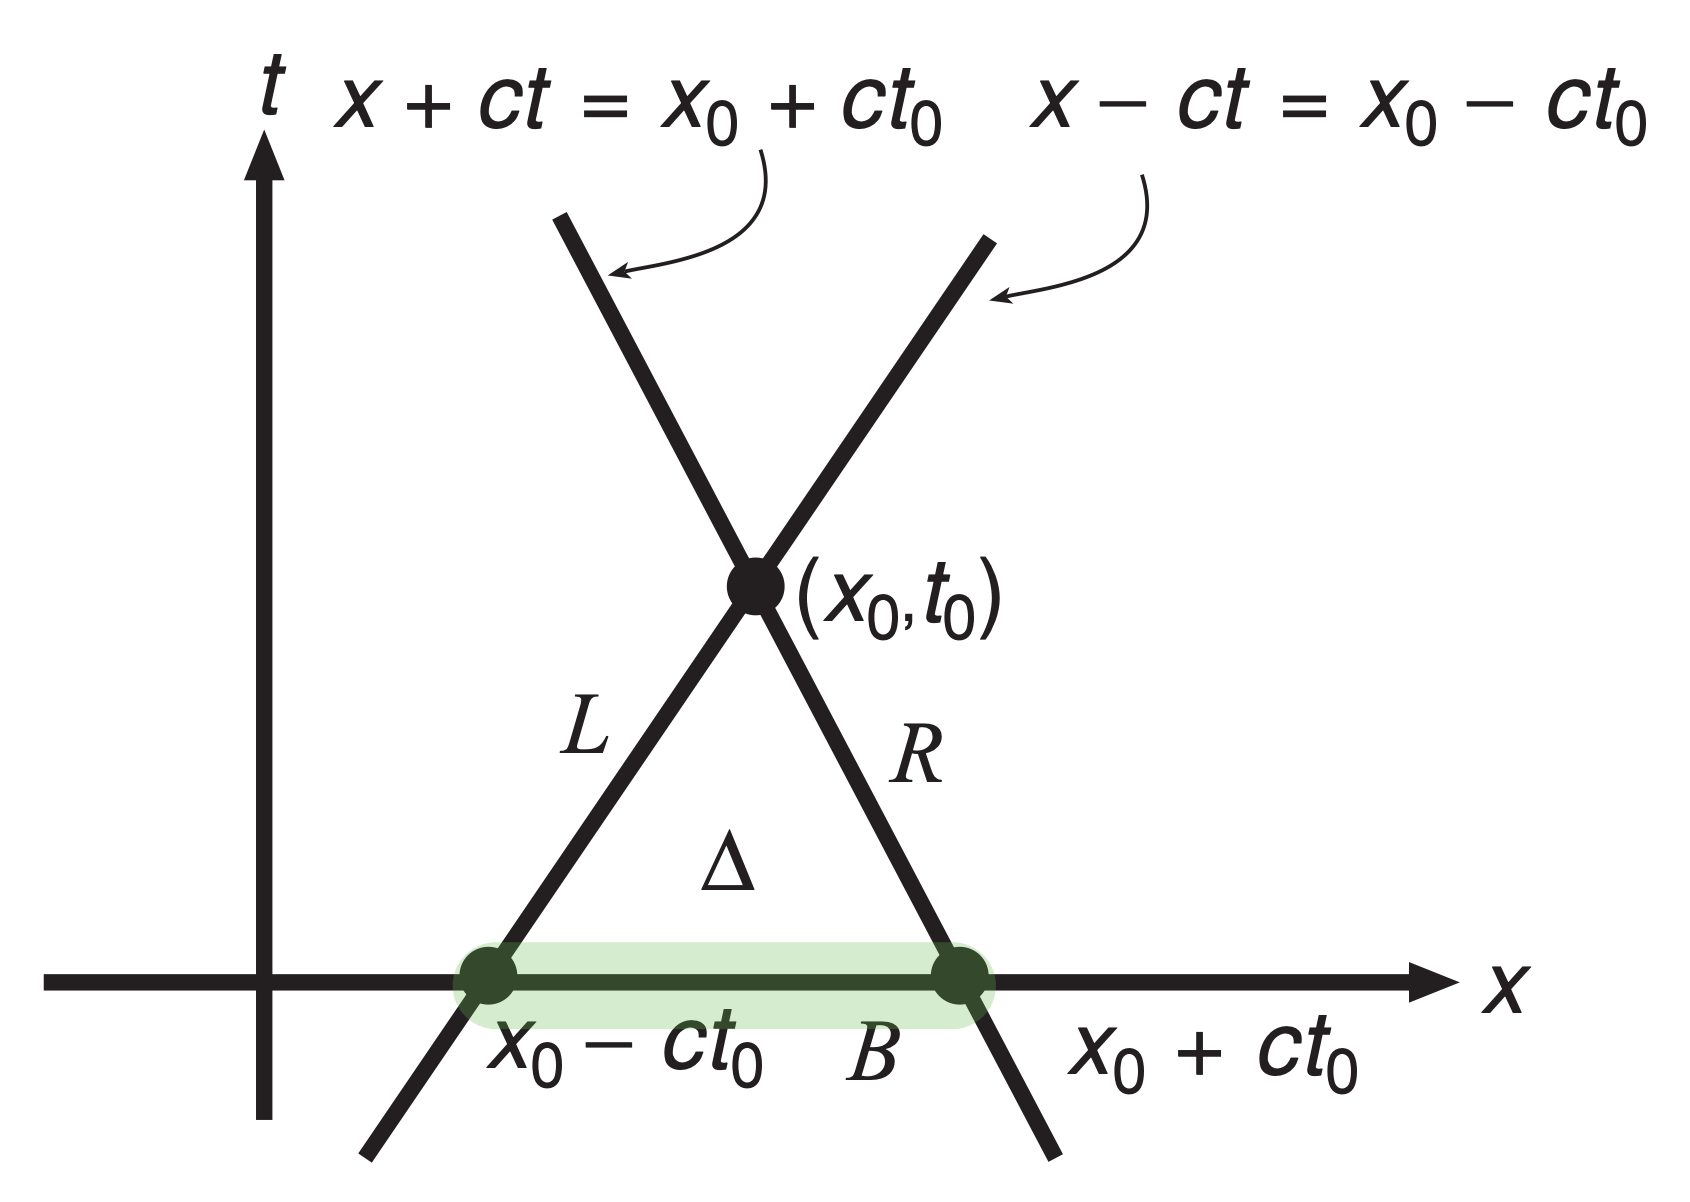
\includegraphics[width=\linewidth]{img/domaindep.png}
\captionof{figure}{Domain of dependence.}
\end{minipage}
\begin{minipage}[h]{0.55\linewidth}
The values at $(x_0,t_0)$ depend only on the initial data at \begin{align*}[a=x_0-ct,b=x_0+ct]\end{align*} Therefore if the initial data live in $[a,b]$ then a point $(x_0,y_0)$ will feel them only if \begin{align*}x_0-ct,x_0+ct]\cap[a,b]\neq\emptyset\end{align*}
\end{minipage}

\subsection{Domain of influence}
\begin{align*}
  \text{DOI} = [x_0-ct,x_0+ct]
\end{align*}

\subsection{Wave equation in interval}
If the problem is stated in an interval $x\in(a,b)$ with zero boundary conditions, a global problem must be found whose solution $\tilde{u}(x,t)$ must coincide with $u$ in the interval. 
\begin{align*}
  \begin{cases}
    \begin{aligned}
      u_{tt} -c^2u_{xx} &= 0 & &(x,t) \in (a,b) \times (0,\infty), \\
      u(a,t) &= 0 & &t \in (0,\infty), \\
      u(b,t) &= 0 & &t \in (0,\infty), \\
      u(x,0) &= f(x) & &x \in (a,b), \\
      u_t(x,0) &= g(x) & &x \in (a,b).
    \end{aligned}
  \end{cases}
\end{align*}
Therefore extend $f(x)$ to be odd with respect to $a$ and $b$. That is
\begin{align*}
  \tilde{u}(-(x-a),t) &= -\tilde{u}((x-a),t) & \tilde{u}(-(x-b),t) &= -\tilde{u}((x-b),t) &
\end{align*}
Then solve the new Cauchy problem:
\begin{align*}
  \begin{cases}
    \begin{aligned}
      \tilde{u}_{tt} -c^2\tilde{u}_{xx} &= 0 & &(x,t) \in \mathbb{R} \times (0,\infty), \\
      \tilde{u}(x,0) &= \tilde{f}(x) & &x \in \mathbb{R}, \\
      \tilde{u}_t(x,0) &= \tilde{g}(x) & &x \in \mathbb{R}.
    \end{aligned}
  \end{cases}
  &&
  u(x,t)&=\tilde{u}(x,t) \quad \text{for} \quad x\in(a,b)
\end{align*}


% -----------------------------------------------------------------------
\section{Separation of variables}
\subsection{Ansatz}
\begin{enumerate}
  \item Write solution as product
    \begin{align*}
      u(x,t)&=X(x)T(t) & u_t(x,t)&=X(x)T'(t) & u_{tt}(x,t)&=X(x)T''(t) \\
      && u_x(x,t)&=X(x)'T(t) & u_{xx}(x,t)&=X(x)''T(t)
    \end{align*}
  \item Substitute into problem
    \begin{align*}
      & u_{t}-u_{xx}=0 &  \frac{T'}{T}=\frac{X''}{X} &= -\lambda = \text{const} &
      &u_{tt}-u_{xx}=0 & \frac{T''}{T}=\frac{X''}{X} &= -\lambda = \text{const}
    \end{align*}
  \item Solve ODE
    \begin{align*}
      X'' &= -\lambda X & \lambda &> 0 & X(x)&=\alpha\sin(\sqrt{\lambda}x)+\beta\cos(\sqrt{\lambda}x) \\
      &&                  \lambda &= 0 & X(x)&=\alpha+\beta x \\
      &&                  \lambda &< 0 & X(x)&=\alpha\sinh(\sqrt{-\lambda}x)+\beta\cosh(\sqrt{-\lambda}x) \\
      &&                          &    & X(x)&=\alpha\sinh(\sqrt{-\lambda}x)+\beta\sinh(\sqrt{-\lambda}(x-\pi)) \\
      T' &= -\lambda T  & &&             T(t)&=e^{-\lambda t}
    \end{align*}
  \item Write $u(x,t)$ as sum and impose initial condition
    \begin{align*}
      u(x,t) &= \sum_{n=0}^\infty X_n(x)T_n(t) & u(x,0) &= \sum_{n=0}^\infty X_n(0)T_n(t)
    \end{align*}
\end{enumerate}

\subsection{Application: Heat equation}
  \begin{align*}
    \begin{cases}
      \begin{aligned}
        u_t - \kappa u_{xx} &= 0, & &0<x<L, t>0,\\
        u(0,t) = u(L,t) &= 0,     & &t\geq0,\\
        u(x,0)  &= f(x),          & &0\leq x\leq L.
      \end{aligned}
    \end{cases}
  \end{align*}

  There exists only a solution for $\lambda > 0$. And hence $u(0,t) = u(L,t) = 0$ the boundary conditions are zero, the $\sin$ is chosen.
  \begin{align*}
    \lambda_n&=\left(\frac{n\pi}{L}\right)^2 & u(x,t)&=\sum_{n=0}^{\infty}B_n\cdot\sin\left(\frac{n\pi}{L}x\right)e^{-\kappa\left(\frac{n\pi}{L}\right)^2t}
  \end{align*}

\subsection{Boundary conditions} \label{ch:boundcond}
  \begin{align*}
    u(0,t)   &= u(L,t)    && \rightarrow \text{Dirichlet} && X_n(x)=\alpha_n\sin(\sqrt{\lambda}x) & 
    \sqrt{\lambda}&=\frac{n\pi}{L}\\
    u_x(0,t) &= u_x(L,t)  && \rightarrow \text{Neumann} && X_n(x)=\alpha_n\cos(\sqrt{\lambda}x) & 
    \sqrt{\lambda}&=\frac{n\pi}{L}\\
    \text{combination}&    && \rightarrow \text{Mixed/Robin} && X_n(x)=\alpha_n\sin((n+\frac{1}{2})\frac{\pi}{L}x) & 
    \sqrt{\lambda}&=\left(n+\frac{1}{2}\right)\frac{\pi}{L}
  \end{align*}

\subsection{Nonhomogeneous case}
  \begin{align*}
    \begin{cases}
      \begin{aligned}
        u_t - u_{xx} &= h(x,t), & &0<x<L, t>0,\\
        u_x(0,t) = u_x(L,t) &= 0,     & &t\geq0,\\
        u(x,0)  &= f(x),          & &0\leq x\leq L.
      \end{aligned}
    \end{cases}
  \end{align*}

  \begin{enumerate}
    \item Check boundary conditions and decide which $X_n(x)$ to use (See \ref{ch:boundcond}). Here Dirichlet is used.
    \item Look for linear combination and make derivatives of $u(x,y)$.
      \begin{align*}
        u(x,t) &= \sum_{n\geq0} T_n(t)cos(\sqrt{\lambda}x) & u_t(x,t) &= \sum_{n\geq0} T_n'(t)cos(\sqrt{\lambda}x) & u_{xx}(x,t) &= \sum_{n\geq0} -\lambda T_n(t)cos(\sqrt{\lambda}x)
      \end{align*}
    \item From the initial condition $u(x,0)=f(x)$ the initial values of $T_n(0)$ can be derived
      \begin{align*}
        u(x,0) &= \sum_{n\geq0} T_n(0)cos(\sqrt{\lambda}x) = f(x) & &\longrightarrow T_n(0)=\dots
      \end{align*}
    \item Imposing $u_t-u_{xx} = h(x,t)$ using the ansatz we get a set of ODE:
      \begin{align*}
        \sum_{n\geq0} (T_n'(t)+\lambda T_n(t) ) cos(\sqrt{\lambda}x) = h(x,t) & &\longrightarrow T_n'(t)=\dots
      \end{align*}
    \item Use $T_n'(t)$ and $T_n(0)$ to solve for all $T_n(t)$
    \item Put solution together
    \item Check solution
  \end{enumerate}

\subsection{Nonhomogeneous boundary conditions}
  \begin{align*}
    \begin{cases}
      \begin{aligned}
        u_t - u_{xx} &= h(x,t), & &0<x<L, t>0,\\
        u_x(0,t) &= a(t),     & &t\geq0,\\
        u_x(L,t) &= b(t),     & &t\geq0,\\
        u(x,0)  &= f(x),          & &0\leq x\leq L.
      \end{aligned}
    \end{cases}
    &&
    \begin{cases}
      \begin{aligned}
        B_a[u]&=\alpha u(a,t)+\beta  u_x(a,t)&=a(t),\ t\geq0 \\ 
        B_b[u]&=\gamma u(b,t)+\delta u_x(b,t)&=b(t),\ t\geq0
      \end{aligned}
    \end{cases}
  \end{align*}

  Find new functino $w(x,t)$ satisfying such non-homogeneous boundary conditions and study the problem being satisfied by $v(x,t)=u(x,t)-w(x,t)$. If the boundary condition is of the following form, table \ref{tab:bound} provides $w(x,t)$.
  \warning\textcolor{red}{Resubstitute to $u(x,t) = v(x,t)+w(x,t)$}
  \begin{center}
    \begin{tabular}{l l l l}
      \hline\hline
      \multicolumn{3}{c}{Boundary condition} & \multicolumn{1}{c}{$w(x,t)$} \\ \hline
      Dirichlet & $u(0,t)=a(t)$   & $u(L,t)=b(t)$   & $w(x,t)=a(t)+\frac{x}{L}[b(t)-a(t)]$ \\
      Neumann   & $u_x(0,t)=a(t)$ & $u_x(L,t)=b(t)$ & $w(x,t)=xa(t)+\frac{x^2}{2L}[b(t)-a(t)]$ \\
      Mixed     & $u(0,t)=a(t)$   & $u_x(L,t)=b(t)$ & $w(x,t)=a(t)+xb(t)$ \\
      Mixed     & $u_x(0,t)=a(t)$ & $u(L,t)=b(t)$   & $w(x,t)=(x-L)a(t)+b(t)$ \\\hline

    \end{tabular}
    \captionof{table}{Boundary conditions} \label{tab:bound}
  \end{center}

\section{Elliptic Equation}
\subsection{Harmonic functions}
Let $D\subset\mathbb{R}^n$. A function $f:D\to\mathbb{R}^n$ is harmonic in $D$ if it is twice differenciable for all $x\in D$. It holds:
\[\Delta f(x)=0\]

\subsection{Poisson equation}
\begin{align*}
  \Delta u &= F(x,y) & 
  \begin{cases}
    \begin{aligned}
      &u(x,y)=g(x,y) &&\text{on} \partial D & &\text{Dirichlet problem} \\
      &\dfrac{\partial u}{\partial v}(x,y)=g(x,y) &&\text{on} \partial D & &\text{Neumann problem} \\
      &U(x,y) + \alpha\dfrac{\partial u}{\partial v}(x,y)=g(x,y) &&\text{on} \partial D & &\text{Robin problem} \\
    \end{aligned}
  \end{cases}
\end{align*}

\textbf{Exists a solution?:} A necessary condition for the existence of a solution to the Neumann problem is
\begin{align*}
  \int_{\partial D}g(x(s))
\end{align*}


\subsection{Definition}
\begin{align*}
  \Delta u = u_{xx} + u_{yy} + u_{zz} &= 0 & \Delta = \dfrac{\partial^2}{\partial x_{1}^2} + \dfrac{\partial^2}{\partial x_{2}^2} + \cdots +\dfrac{\partial^2}{\partial x_{n}^2}
\end{align*}

\subsection{Maximum Principle}
\textbf{weak maximum principle:} Let $D$ be a bounded domain, and let $u(x,y)\in C^2(D)\cap C(\bar{D})$ be a harmonic function in $D$. Then the maximum of $u$ in $\bar{D}$ is achieved on the boundary $\partial D$. If $u$ is harmonic in $D$, then $-u$ is harmonic there too. Therefore the minimum of a harmonic function $u$ is also obtained on the boundary $\partial D$.
\begin{align*}
  \max_{\bar{D}} u &= \max_{\partial D} u & \min_{\bar{D}} u &= \min_{\partial D} u
\end{align*}

\textbf{strong maximum principle:} Let $u$ be a harmonic function in a domain $D$. If $u$ attains its maximum (minimum) at an interior point of $D$, then $u$ is constant.

\subsection{Mean value Principle}
Let $(x_0,y_0)$ be a point in $D$. Assume that $B_R$ is a disk of radius $R$ centered at $(x_0,y_0)$, fully contained in $D$. For any $r>0$ set $C_r=\partial B_r$. Then the value of u at $(x_0,y_0)$ is the average of the values of $u$ on the circle $C_R$:
\begin{align*}
  u(x_0,y_0)  &= \frac{1}{2\pi R} \oint_{C_R}u(x(s),y(s))\mathrm{d}s \\
              &= \frac{1}{2\pi} \int_{0}^{2\pi}u(x_0+R\cos(\theta),y_0+R\sin\theta)\mathrm{d}\theta
\end{align*}

\subsection{General uiniqueness for Poisson eq.}
From Theorem (7.12):
\begin{enumerate}
  \item Let $v=u_1-u_2$ ($u_1$ and $u_2$ are soltutions to the poisson eq.)
  \item Take a point $(x_0,y_0)$ and propose $v(x_0,y_0) = M > 0$
  \item Show by writing $0=\Delta v(x_0,y_0) -kv(x_0,y_0) \leq -kM$ a contradiction $\to v(x_0,y_0) \nless 0$
  \item Take a point $(x_1,y_1)$ and propose $v(x_1,y_1) = M < 0$
  \item Show by writing $0=\Delta v(x_1,y_1) -kv(x_1,y_1) \geq -kM$ a contradiction $\to v(x_1,y_1) \ngtr 0$
  \item Using \textit{weak max principle} it holds that $v=0 \iff u_1=u_2$
\end{enumerate}

\subsection{Laplace equation in rectangular domain}
\begin{minipage}[h]{0.6\linewidth}
  \begin{align*}
    \begin{cases}
      \begin{aligned}
        \Delta u &= 0, & &(x,y) \in (a,b) \times (c,d), \\
        u(a,y), &= f(y) & &c < y < d, \\
        u(b,y), &= g(y) & &c < y < d, \\
        u(x,c), &= h(x) & &a < x < b, \\
        u(x,d), &= k(x) & &a < x < b. 
      \end{aligned}
    \end{cases}
  \end{align*}
\end{minipage}
\begin{minipage}[h]{0.35\linewidth}
  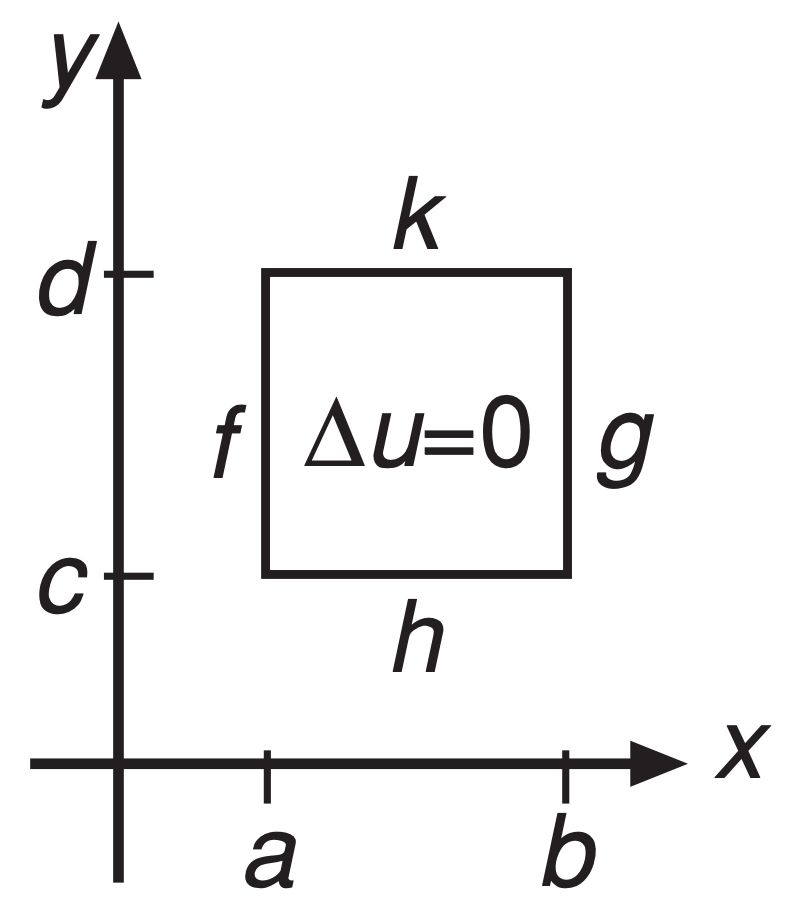
\includegraphics[width=0.5\linewidth]{img/rect.png}
  \captionof{figure}{Separation of variables in rectangles.}
\end{minipage}

\textbf{Neumann $\exists$ sol. if:} For $u_x()/u_y()$. The neccessary condition must hold that the integral over the boundary is zero. \warning\textcolor{red}{Mind the integral limits/direction}
  \begin{align*}
    0 = -\Int_a^bh\mathrm{d}x+\Int_c^dg\mathrm{d}y+\Int_a^bk\mathrm{d}x-\Int_c^df\mathrm{d}y
      % 0 = \int_{\partial D} \frac{\partial u}{\partial v} = 
      % \Int^c_dg(s)\mathrm{d}s+ \Int^b_ak(s)\mathrm{d}s+\Int^d_cf(s)\mathrm{d}s+ \Int^a_bh(s)\mathrm{d}s
  \end{align*}

\textbf{Ansatz:} $u(x,y)=X(x)Y(y)$ For $X(x)$ proceed as in \ref{ch:boundcond}. For $Y(y)$ The following are equivalent:
  \begin{align*}
    Y_n(y) &= A_n \sinh(\sqrt{\lambda}y) + B_n \sinh(\sqrt{\lambda}y & &\\
           &= C_n \sinh(\sqrt{\lambda}(y-c)) + D_n \sinh(\sqrt{\lambda}(y-d)) & &\\
           &= E_n \cosh(\sqrt{\lambda}(y-c)) + F_n \cosh(\sqrt{\lambda}(y-d)) & &\\
           &= G_n \cosh(\sqrt{\lambda}(y-c)) + H_n \sinh(\sqrt{\lambda}(y-d)) & &\\
           &= J_n \cosh(\sqrt{\lambda}y) + K_n \cosh(\sqrt{\lambda}y) & &\leftarrow\text{ use this if $u_x/u_y$ is given}
  \end{align*}
Most common:
\begin{align*}
  \eqbox{Y_0(y) = \alpha_0y+\beta_0, \quad Y_n(y) = \alpha_n \sinh(\sqrt{\lambda}(y-c)) + \beta_n \sinh(\sqrt{\lambda}(y-d)) \quad n \geq 1}
\end{align*}
Then use the following and introduce boundaries $u(x,c)$ and $u(x,d)$.
\begin{align*}
  \eqbox{u(x,y) = \alpha_0y+\beta_0+\sum_{n\leq1}\cos(\sqrt{\lambda}x)\left[\alpha_n\sinh(\sqrt{\lambda}(y-c))+\beta_n\sinh(\sqrt{\lambda}(y-d))\right]}
\end{align*}

\subsection{Laplace eq. in circular domain}
  Problem:
  \begin{align*}
    &\begin{cases}
      \Delta u = 0, & \text{in} \quad D,\\
      u(r_a,\theta) = f(\theta), & \text{for} \quad 0 \leq \theta \leq 2\pi,\\
      u(r_b,\theta) = g(\theta), & \text{for} \quad 0 \leq \theta \leq 2\pi.
    \end{cases}
    &
    \Delta &= \frac{\partial^2}{\partial r^2} \frac{1}{r}\frac{\partial}{\partial r} + \frac{1}{r^2} \frac{\partial^2}{\partial \theta^2}
  \end{align*}

  Ansatz: If the boundary datum depends only on sine, the sine only ansatz can be chosen. \textcolor{red}{Provide reason!} Then introduce boundary conditions and solve for $A_n,B_n, \dots$
  \begin{align*}
    \text{General} && u(t,\theta) &= \sum_{n>0}\left(A_nr^n+B_nr^{-n}\right)\sin(n\theta) + C_0 + D_0\log(r) \\
                               && &+ \sum_{n>0}\left(C_nr^n+D_nr^{-n}\right)\cos(n\theta) \\
    \text{sin only} && u(t,\theta) &= \sum_{n>0}\left(A_nr^n+B_nr^{-n}\right)\sin(n\theta) \\
    \text{cos only} && u(t,\theta) &= \sum_{n>0}\left(C_nr^n+D_nr^{-n}\right)\cos(n\theta) + C_0 + D_0\log(r)
  \end{align*}

  If origin ($r=0$) is inside domain $D$ then $D_n=D_0=0 \quad \forall n$ because $r^{-n}$ and $\log(r)$ blow up for $r\to0$.


% -----------------------------------------------------------------------
% 
% -----------------------------------------------------------------------
\vfill\null
\columnbreak
\section{Common Tables}
\subsection{Derivatives and Integrals}
  \begin{align*}
        &[c]' = 0  &&\int0\mathrm{d}x = c \\
        &[x]' = 1 && \int1 \mathrm{d}x = x+c\\
        &[x^{n+1}]' = (n+1)x^n, n\neq-1 && \int x^n \mathrm{d}x = \frac{1}{n+1}x^{n+1}+x, n\neq -1\\
        &[\ln x]' = \frac{1}{x}, x>0 && \int \frac{1}{x}\mathrm{d}x = ln|x|+c\\
        &[\ln(-x)]' = \frac{-1}{-x}=\frac{1}{x},x<0 &&\int\frac{1}{x}\mathrm{d}x = ln|x|+c \\
        \cline{1-4}
        &[e^x]' = e^x && \int e^x \mathrm{d}x = e^x + c\\
        &[a^x]' = a^x\ln a && \int a^x \mathrm{d}x = \frac{1}{\ln a}a^x + c, a \neq 1\\
        \cline{1-4}
        &[\sin x]' = \cos x && \int \cos x \mathrm{d}x = \sin x + x\\
        &[\cos x]' = -\sin x && \int \sin x \mathrm{d}x = -\cos x + x\\
        &[\tan x]' = \frac{1}{\cos^2 x} = 1 + \tan^2x && \int \frac{1}{\cos^2x}\mathrm{d}x = \tan x + c\\
        & && \int \tan^2x\mathrm{d}x = \tan x - x+ c\\
        &[\cot x]' = -\frac{1}{\sin^2x} = -1-\cot^2x && \int \frac{1}{\sin^2x}\mathrm{d}x = -\cot x + c\\
        & && \int \cot^2x\mathrm{d}x = -\cot x - x + c\\
        \cline{1-4}
        &[\arcsin x]' = \frac{1}{\sqrt{1-x^2}} && \int \frac{1}{\sqrt{1-x^2}} \mathrm{d}x = \arcsin x + c_1\\
        &[\arccos x]' = -\frac{1}{\sqrt{1-x^2}} && \int \frac{1}{\sqrt{1-x^2}} \mathrm{d}x = -\arccos x + c_2\\
        &[\arctan x]' = \frac{1}{1+x^2} && \int \frac{1}{1+x^2} \mathrm{d}x = \arctan x + c_1\\
        &[\mathrm{arccot} x]' = -\frac{1}{1+x^2} && \int \frac{1}{1+x^2} \mathrm{d}x = \mathrm{arccot} x + c_2\\
        \cline{1-4}
        &[\sinh x]' = \cosh x  &&\int \cosh x \mathrm{d}x = \sinh x + c \\
        &[\cosh x]' = \sinh x  &&\int \sinh x \mathrm{d}x = \cosh x  + c \\
        &[\tanh x]' = \frac{1}{\cosh^2x} = 1-\tanh^2x  &&\int \frac{1}{\cosh^2x} \mathrm{d}x = \tanh x + c \\
        &[\coth x]' = -\frac{1}{\sinh^2x} =1-\coth^2x &&\int \frac{1}{\sinh^2x} \mathrm{d}x = -\coth x  + c \\
        \cline{1-4}
  \end{align*}
  \begin{align*}
        &[\mathrm{arsinh}x]' =  \frac{1}{\sqrt{x^2+1}} &&\int \frac{1}{\sqrt{x^2+1}} \mathrm{d}x = \mathrm{arsinh}x  + c = \ln(x+\sqrt{x^2+1}) \\
        &[\mathrm{arcosh}x]' =  \frac{1}{\sqrt{x^2-1}} &&\int \frac{1}{\sqrt{x^2-1}} \mathrm{d}x = \mathrm{arcosh}x  + c = \ln(x+\sqrt{x^2-1}) \\
        &[\mathrm{artanh}x]' = \frac{1}{\sqrt{1-x^2}},|x|<1 &&\int \frac{1}{\sqrt{1-x^2}},|x|<1 \mathrm{d}x = \mathrm{artanh}x+c=\frac{1}{2}\ln\frac{1+x}{1-x}+c,|x|<1  + c \\
        &[\mathrm{arcoth}x]' = \frac{1}{\sqrt{1-x^2}},|x|>1 &&\int \frac{1}{\sqrt{1-x^2}} \mathrm{d}x = \mathrm{arcoth}x+c=\frac{1}{2}\ln\frac{x+1}{x-1}+c,|x|>1 + c \\
        \cline{1-4}
        &\int \sin^2(x) \mathrm{d}x = - \frac{1}{4}\sin(2x) +\frac{1}{2}x+c && \int \cos^2(x) \mathrm{d}x = \frac{1}{4}\sin(2x) +\frac{1}{2}x+c
  \end{align*}

\subsection{Derivative rules}
\begin{align*}
  (f+g)' &= f'+g' & (cf)' &= cf' & (fg)' &= f'g + g'f \\
  (\frac{f}{g})' &= \frac{f'g-fg'}{g^2} 
\end{align*}

\subsection{Integral rules}
\begin{align*}
  &\text{substitution}      & &\int_{a}^{b}f[u(x)]u'(x)\mathrm{d}x = \int_{u(a)}^{u(b)}f(z)\mathrm{d}z \quad z = u(x) \\
  &\text{partial integral}  & &\int_a^b u(x)v'(x)\mathrm{d}x=u(x)v(x)|_a^b-\int_a^bu'(x)v(x)\mathrm{d}x
\end{align*}

\subsection{Trigonometric identities}
\begin{align*}
  & \sin(x) = \frac{e^{ix}-e^{-ix}}{2i} && \cos(x) = \frac{e^{ix}+e^{-ix}}{2} \\
  & \sin^2(x) + \cos^2(x) = 1 && \sin(\alpha+\beta)=\sin(\alpha)\cos(\beta)+\sin{\beta}\cos(\alpha) \\
  & \cos(2x) = \cos^2(x)-\sin^2(x) && \sin(\alpha-\beta)=\sin(\alpha)\cos(\beta)-\sin{\beta}\cos(\alpha) \\
  & \sin(2x) = 2\sin(x)\cos(x) && \cos(\alpha+\beta)=\cos(\alpha)\cos(\beta)-\sin{\alpha}\sin(\beta) \\
  & c^2=a^2+b^2-2ab\cos(\gamma) && \cos(\alpha-\beta)=\cos(\alpha)\cos(\beta)+\sin{\alpha}\sin(\beta) \\
  & \frac{a}{\sin{\alpha}}=\frac{b}{\sin{\beta}}=\frac{c}{\sin{\gamma}} && \cos^2(x) = \frac{1+\cos(2x)}{2}
\end{align*}

\subsection{Hyperbolic identities}
\begin{align*}
  & \sinh(x) = \frac{e^{x}-e^{-x}}{2} && \cosh(x) = \frac{e^{x}+e^{-x}}{2} \\
  & \cosh^2(x) - \sinh^2(x) = 1 && \sinh(x\pm y)=\sinh(x)\cosh(y)\pm\sinh{y}\cosh(x) \\
  & \sinh(2x) =2\sinh(x)\cosh(x) && \cosh(x\pm y)=\cosh(x)\cosh(y)\pm\sinh{x}\sinh(y) \\
  & \cosh(2x) =\cosh^2(x) + \sinh^2(x) && \\
  & \sinh(-x) =-\sinh{x} && \\
  & \cosh(-x) = \cosh{x} && \\
\end{align*}

\subsection{Sums}
\begin{align*}
\sum_{k=1}^{n}k&=\frac{n(n+1)}{2} & \sum_{k=1}^{n}k^2&=\frac{n(n+1)(2n+1)}{6} & \sum_{k=1}^{n}k^3 &= \frac{n^2(n+1)^2}{4} \\
\sum_{k=0}^{n-1}q^{k}&=\frac{1-q^n}{1-q} & \sum_{k=0}^{\infty}q^k&=\frac{1}{1-q}, \text{for}|q|<1 & \binom{n}{k} &= \frac{n!}{k!(n-k)!}
\end{align*}





\vspace*{\fill}
% You can even have references
\rule{0.3\linewidth}{0.25pt}\\
Good Luck!
%\scriptsize
%\bibliographystyle{abstract}
%\bibliography{refFile}
\end{multicols*}
\end{document}
